\chapter{Porting Tang}\label{porting-tang}

After successfull cross-compilation of jose we have all the dependencies "ready" and packaged except the systemd.
systemd is only one of the many implementations (inetd, launchd, ucspi-tcp, xinetd) of a super-server providing socket activation.

\section{Socket activation}

Socket activation is a technology provided by a super-server (also called a service dispatcher daemon).
A super-server starts other servers when needed as well, normally with access to them checked by a TCP wrapper.
It uses very few resources when in idle state.

A service designed for the socket activation would behave as bare CLI application with input read from stdin (standard input) and output written to stdout (standard output).
Tang is exactly this kind of an application and because of that we need to configure socket activation\cite{super_server}.



\subsection{xinetd}
xinetd listens for incoming requests over a network and launches the appropriate service for that request.
Requests are made using port numbers as identifiers and xinetd usually launches another daemon to handle the request.
This is reflected on Figure \ref{fig_xinetd} xinetd socket activation below.
\begin{figure}[h]
    \centering
    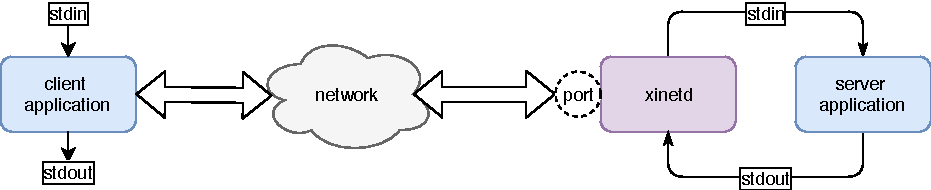
\includegraphics[scale=0.9]{figures/xinetd.pdf}
    \caption{xinetd socket activation}
    \label{fig_xinetd}
\end{figure}
xinetd features access control mechanisms such as TCP Wrapper ACLs (access control lists), extensive logging capabilities, and the ability to make services available based on time.
It can place limits on the number of servers that the system can spawn.
xinetd is listening on behalf of the services.
Whenever a connection would come in an instance of the respective service will be spawned with using stdin and stdout of the service application\cite{xinetd}.



\section{Install dependencies}

As we have all of the Tang dependencies "ready"

update feeds
feeds install
make menuconfig
\newpage



to have an example created simple application in C for xinetd
\newpage

\section{Cross-compile Tang}

do not forget to add xinetd in Dependencies
\newpage

\subsection{Hurdles with http-parser}\label{http_parser_problems}

without upstream patch not working tang
\newpage

\subsection{Mysterious José}

does makefiles support shell {a,b} thing???
\newpage

\section{Configure Tang with xinetd}

We need xinetd's socket activation for Tang to work.


there is no systemd for OpenWrt

/etc/services

xinetd configuration

\subsection{}


% root@A04-0315A:~# if [ -z "$(find /usr/share/tang/db/ -name "*.jw*" -maxdepth 1)" ]; then echo nic; else echo daco;fi
% daco
% root@A04-0315A:~# if [ -z "$(find /usr/share/tang/db/ -name "*.jwk" -maxdepth 1)" ]; then echo nic; else echo daco;fi
% daco
